
\documentclass[12pt, a4paper,
oneside
openany
]{report}

%% Nutné balíčky a nastavení
%%%%%%%%%%%%%%%%%%%%%%%%%%%%

%% Proměnné
\newcommand\obor{INFORMAČNÍ TECHNOLOGIE} %% -- napiš číslo a název tvého oboru
\newcommand\kodOboru{18-20-M/01} %% -- napiš číslo a název tvého oboru
\newcommand\zamereni{se zaměřením na počítačové sítě a programování} %% -- napiš číslo a název tvého oboru
\newcommand\skola{Střední škola průmyslová a umělecká, Opava} %% vyplň název školy
\newcommand\trida{IT4} %% vyplň jméno svého konzultanta
\newcommand\jmenoAutora{Robin Harazim}  %% vyplň své jméno
\newcommand\skolniRok{2023/24} %% vyplň rok
\newcommand\datumOdevzdani{1. 1. 2024} %% vyplň rok
\newcommand\nazevPrace{Tank na dálkové ovládání TM-1} %% vyplň název své práce

\title{\nazevPrace} %% -- Název tvé práce
\author{\jmenoAutora} %% -- tvé jméno
\date{\datumOdevzdani} %% -- rok, kdy píšeš SOČku

\usepackage[top=2.5cm, bottom=2.5cm, left=3.5cm, right=1.5cm]{geometry} %% nastaví okraje, left -- vnitřní okraj, right -- vnější okraj

\usepackage[czech]{babel} %% balík babel pro sazbu v češtině
\usepackage[utf8]{inputenc} %% balíky pro kódování textu
\usepackage[T1]{fontenc}
\usepackage{cmap} %% balíček zajišťující, že vytvořené PDF bude prohledávatelné a kopírovatelné

\usepackage{graphicx} %% balík pro vkládání obrázků

\usepackage{subcaption} %% balíček pro vkládání podobrázků

\usepackage{hyperref} %% balíček, který v PDF vytváří odkazy

\linespread{1.5} %% řádkování
\setlength{\parskip}{0.5em} %% odsazení mezi odstavci


\usepackage[pagestyles]{titlesec} %% balíček pro úpravu stylu kapitol a sekcí
\titleformat{\chapter}[block]{\scshape\bfseries\LARGE}{\thechapter}{10pt}{\vspace{0pt}}[\vspace{-22pt}]
\titleformat{\section}[block]{\scshape\bfseries\Large}{\thesection}{10pt}{\vspace{0pt}}
\titleformat{\subsection}[block]{\bfseries\large}{\thesubsection}{10pt}{\vspace{0pt}}


\usepackage{tocloft} % Balíček umožní přizpůsobit vzhled tabulky obsahu
\setlength{\cftbeforechapskip}{0pt}  % Menší rozestup pro kapitoly
\setlength{\cftbeforesecskip}{0pt}   % Menší rozestup pro sekce

\setcounter{secnumdepth}{2}
\setcounter{tocdepth}{3}
\usepackage{fancyhdr}
\pagestyle{fancy}
\renewcommand{\headrulewidth}{0.025pt}

\usepackage{booktabs}

\usepackage{url}

%% Balíčky co se můžou hodit :) 
%%%%%%%%%%%%%%%%%%%%%%%%%%%%%%%

\usepackage{pdfpages} %% Balíček umožňující vkládat stránky z PDF souborů, 

\usepackage{upgreek} %% Balíček pro sazbu stojatých řeckých písmen, třeba u jednotky mikrometr. Například stojaté mí: \upmu, stojaté pí: \uppi

\usepackage{amsmath}    %% Balíčky amsmath a amsfonts 
\usepackage{amsfonts}   %% pro sazbu matematických symbolů
\usepackage{esint}     %% pro sazbu různých integrálů (např \oiint)
\usepackage{mathrsfs}
\usepackage{helvet} % Helvet font
\usepackage{mathptmx} % Times New Roman
\usepackage{Oswald} % Oswald font


%% makra pro sazbu matematiky
\newcommand{\dif}{\mathrm{d}} %% makro pro sazbu diferenciálu, místo toho
%% abych musel psát '\mathrm{d}' mi stačí napsat '\dif' což je mnohem 
%% kratší a mohu si tak usnadnit práci

\usepackage{listings}
\usepackage{xcolor}
\usepackage{varwidth}
\usepackage{ragged2e}


\definecolor{codegreen}{rgb}{0,0.6,0}
\definecolor{codegray}{rgb}{0.5,0.5,0.5}
\definecolor{codepurple}{rgb}{0.58,0,0.82}
\definecolor{backcolour}{rgb}{0.95,0.95,0.92}

\lstdefinestyle{arduinoStyle}{
    language=C++,
    backgroundcolor=\color{backcolour},   
    commentstyle=\color{codegreen},
    keywordstyle=\color{blue},
    numberstyle=\tiny\color{codegray},
    stringstyle=\color{codepurple},
    basicstyle=\ttfamily\small,
    breakatwhitespace=false,         
    breaklines=true,                 
    captionpos=b,                    
    keepspaces=true,                 
    numbers=left,                    
    numbersep=5pt,                  
    showspaces=false,                
    showstringspaces=false,
    showtabs=false,                  
    tabsize=2,
    frame=single,
    framesep=5pt,
    framexleftmargin=5mm,
    rulecolor=\color{black},
    xleftmargin=10mm,
    morekeywords={digitalWrite, setup, loop, rotateMotor}, 
    identifierstyle=\color{codepurple} 
}


%% Bordel pro práci - můžeš smáznout :) 
%%%%%%%%%%%%%%%%%%%

\usepackage{lipsum} %% balíček který píše lipsum (nesmyslný text, který se používá pro kontrolu typografie)

%% Začátek dokumentu
%%%%%%%%%%%%%%%%%%%%
\begin{document}
	
    \setcounter{page}{1}
    \pagestyle{empty}

%% Titulní stránka s informacemi
%%%%%%%%%%%%%%%%%%%%%%%%%%%%%%%%%%%%%%%%
	
	{\fontfamily{phv}\selectfont
		%% Logo školy
		\begin{figure}[h]
			\centering
			
\includegraphics[width=0.6\linewidth]{image/logo-skoly.png} 
		\end{figure}
		
		
		%% Hlavička práce a její název (viz proměnná \nazev prace)
		%% \sffamily %%% bezpatkové písmo - sans serif
		{\bfseries %%% písmo na stránce je tučně
			\begin{center}
				\vspace{0.025 \textheight}
				\LARGE{ZÁVĚREČNÁ STUDIJNÍ PRÁCE}\\
				\large{dokumentace}\\
				\vspace{0.075 \textheight}
				\LARGE {\nazevPrace}\\
			\end{center}  
		}%%%
		
		\begin{figure}[ht]
			\centering
			
\includegraphics[width=0.8\linewidth]{image/programovani-02.jpg} 
		\end{figure}
		
		\vspace{0.02 \textheight}
		\begin{table}[h!]
			\begin{tabular}{ll}
				\textbf{Autor:} & \jmenoAutora\\ 
				\textbf{Obor:} & \kodOboru { } \obor\\
				\textbf{} & \zamereni\\
				\textbf{Třída:} & \trida\\
				\textbf{Školní rok:} & \skolniRok\\
			\end{tabular}
			
		\end{table}		
	}
	
	
%% Stránka obsahující poděkování a prohlášení
%%%%%%%%%%%%%%%%%%%%%%%%%%%%%%%%%%%%%%%%%%%%%%%%%%%%%%%%

%% Poděkování - nepovinné
%%%%%%%%%%%%%%%%%%%%%%%%%%%%
    \newpage
    \noindent{\large{\bfseries{Poděkování}\\}}
    \noindent Chtěl bych  poděkovat panu učiteli Mgr. Marcelu Godovskému za poskytnutí 3D tisku a užitečné rady při vytváření projektu.


	\vspace*{0.6\textheight} %% Vertikální mezeru je možné upravit




%% Prohlášení - povinné
%%%%%%%%%%%%%%%%%%%%%%%%%%%%
	\noindent{\large{\bfseries{Prohlášení}\\}}  %% uprav si koncovky podle toho na jaký rod se cítíš, vypadá to pak lépe :) 
	\noindent{Prohlašuji, že jsem závěrečnou práci vypracoval samostatně a uvedl veškeré použité 
		informační zdroje.\\}
	\noindent{Souhlasím, aby tato studijní práce byla použita k výukovým a prezentačním účelům na Střední průmyslové a umělecké škole v Opavě, Praskova 399/8.}
	\vfill
	\noindent{V Opavě \datumOdevzdani\\}
	\noindent
	\begin{minipage}{\linewidth}
		\hspace{9.5cm} 
		\begin{tabular}{@{}p{6cm}@{}}
			\dotfill \\
			Podpis autora
		\end{tabular}
	\end{minipage}
	
	\clearpage %% Zalomení dvojstránky

%% Stránka obsahující abstrakt (anotaci)
%%%%%%%%%%%%%%%%%%%%%%%%%%%%%%%%%%%%%%%%%%%%%%%%%%%%%%%%	

%% Abstrakt v češtině
%%%%%%%%%%%%%%%%%%%%%%%%%%%%
	\noindent{\Large{\bfseries{Abstrakt}\\}}
    	\noindent Tato práce se zaměřuje na konstrukci dálkově ovládaného tanku, jehož většina součástek byla vyrobena technologií 3D tisku. Základní řídící jednotkou je vývojová deska ESP32 s vestavěnou kamerou a WiFi modulem, která umožňuje živé ovládání tanku prostřednictvím webového serveru postaveného na knihovně ESPAsyncWebServer. Webové rozhraní dává uživatelům možnost sledovat tank v reálném čase, což značně usnadňuje jeho ovladatelnost. Součástí projektu je také sestrojení vlastního ovladače jako možnost alternativního ovládání. \\
	
	\vspace{18pt}
	
	\noindent{\large{\bfseries{Klíčová slova}}}
	
	\noindent ESP32, Tank, závěrečná práce, dokumentace, \dots 
	
	
	\clearpage %% Zalomení stránky

%% Stránka s generovaným obsahem
%%%%%%%%%%%%%%%%%%%%%%%%%%%%%%%%%%%%%%%


\fancypagestyle{originalplain}{
  \fancyhf{}
  \fancyfoot[C]{\thepage} 
  \renewcommand{\headrulewidth}{0pt}
  \renewcommand{\footrulewidth}{0pt}
}


\fancypagestyle{plain}{
  \fancyhf{} 
  \renewcommand{\headrulewidth}{0pt}
  \renewcommand{\footrulewidth}{0pt}
}

\pagestyle{empty} 
	\tableofcontents 
 
%% Stránka s úvodem - povinná část
%%%%%%%%%%%%%%%%%%%%%%%%%%%%%%%%%%%%%%%	
	\chapter*{Úvod}
	\addcontentsline{toc}{chapter}{Úvod}
 \fancypagestyle{plain}{%

  \fancyhf{}
  \fancyfoot[C]{\thepage} 
  \renewcommand{\headrulewidth}{0pt}
  \renewcommand{\footrulewidth}{0pt}
}
    \pagestyle{plain}
 
\noindent Mou hlavní motivací pro tento projekt byla má dlouhodobá záliba ve vojenské technice, jenž se se mnou táhne již od dětství a také zájem v oblasti hardware. Rozhodl jsem se tedy tyto své dvě záliby zkombinovat a vytvořit tak tento projekt. \\
Cílem této práce bylo tedy vytvořit tank na dálkové ovládání s možností ovládání přes webový server nebo přes vlastnoručně vyrobený ovladač.
Při vytváření mého projektu jsem se nejprve musel rozhodnout, které součástky budou nejvhodnější, a zároveň jsem pečlivě promýšlel, zda si vybrat předem sestavený model nebo se pustit do výroby vlastních komponentů a jejich následného 3D tisku.\\
Původně jsem zamýšlel všechny díly sám vymodelovat, ale vzhledem k tomu, že toto řešení by bylo docela dost časově náročné, rozhodl jsem se najít si na internetu vhodný model podvozku i s pásy a zbytek domodelovat sám. Všechny díly jsem nakonec vytiskl na 3D tiskárně a smontoval dohromady.\\
Jako jádro projektu jsem si zvolil právě vývojovou desku ESP32, vybavenou integrovaným Wi-Fi modulem a kamerou, a jako první jsem chtěl vytvořit jednoduchý webový server pomocí knihovny ESPAsynchWebServer, který by umožňoval připojenému uživateli tank ovládat pomocí živého obrazu z kamery na serveru. Další problematikou by bylo sestrojení vlastního ovladače jako alternativní možnost pro ovládání tanku.\\
V této dokumentaci se tedy snažím podrobněji popsat svůj postup při řešení projektu a také problémy se kterými jsem se setkal a jejich řešení. 

\chapter{Využité technologie}

\section{Technologie 3D tisku}
\noindent Technologie 3D tisku představuje revoluční způsob výroby, který umožňuje vrstvení materiálů a vytváření trojrozměrných objektů podle digitálních modelů. Jednou z hlavních výhod této technologie je schopnost tvořit vrstvením, což znamená postupné nanášení materiálu podle přesného digitálního modelu. To přináší nejen efektivní výrobu, ale také možnost přizpůsobit design součástek dle konkrétních požadavků. Proces využívá 3D modelovací software pro vytváření designů a slicer software k přípravě dat pro tisk. Tiskárna postupně nanáší a vrství materiál, často termoplastický filament, a vytváří tak fyzický objekt. Tato technologie nachází široké uplatnění v průmyslu, od výroby prototypů přes modelářství až po vytváření funkčních součástek pro stroje a zařízení. Já se taktéž rozhodl využít tuto technologii ve svém projektu. Nejprve jsem chtěl všechny součástky sám vymodelovat, ale nakonec jsem přistoupil na kompromis vlastní výroby a již předem vymodelovaného projektu, který jsem si našel na internetu.

\section{Hardware}
\label{sec:zakladni_struktura}

V této kapitole se budu podrobně věnovat představení klíčových součástek, které jsem ve svém projektu využil.

\newpage

\subsection{Seznam součástek}

\begin{itemize}
  \item Vývojová deska ESP32-CAM, WiFi + Bluetooth
  \item H-můstek L298N, dvoumotorový modul
  \item 2x Plastové micro servo SG90 9g, 180°
  \item Součástky vytvořené pomocí 3D tisku
  \item Napájecí modul
  \item Nepájivé pole
\end{itemize}

\subsection{Vývojová deska ESP32-CAM}
\noindent V mém projektu hraje klíčovou roli vývojová deska ESP32-CAM, která se stala nezbytným jádrem celého systému, jelikož na ní běží webový server, bez kterého by nebylo možné tank ovládat a také program pro pohyb tanku. Tato kompaktní vývojová deska od společnosti Espressif Systems kombinuje WiFi a Bluetooth komunikaci s kamerovým modulem OV2640 schopným snímání obrázků s rozlišením až 2 megapixely. Obsahuje celkem 10 digitálních GPIO pinů, a pro program je k dispozici pamět o celkové velikosti 128kB. Deska taktéž pracuje s napětím 5 V, což zajišťuje bezproblémovou integraci s dalšími součástkami projektu. 

	\begin{figure}[ht]
		\centering 
		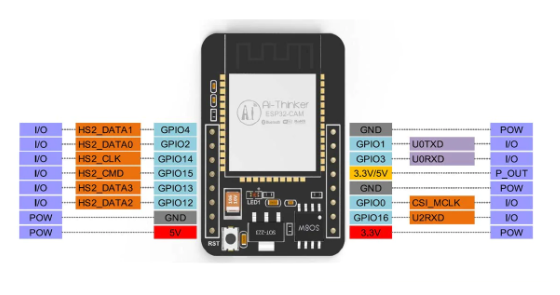
\includegraphics[width=0.7\textwidth]{image/esp-detail} %
		\caption{Vývojová deska ESP32-CAM \cite{ESP32}.} 
	\end{figure}

\subsection{H-můstek L298N}
\noindent H-můstek L298N je integrovaný obvod, který slouží jako řadič pro motory. Je široce využíván v elektronických projektech, zejména v robotice a modelářství. Tento můstek umožňuje kontrolu směru otáčení a rychlosti stejnosměrných motorů. Modul využívá výkonný čip ST L298N a zaručuje taktéž ochranou proti zkratu a přehřátí. Jeho konstrukce obsahuje dva H-můstky, což znamená, že může řídit až dva motory nezávisle na sobě. Tato komponenta poskytuje efektivní řešení pro pohonný systém v různých elektronických aplikacích. Jeho vestavěný 5V stabilizátor umožňuje kompatibilitu s dalšími komponenty mého projektu. V mém projektu jsem tento H-můstek využil k ovládání motorů. Jeho úlohou je převádět vstupní signály, které přicházejí ze serveru, na konkrétní směr otáčení motorů.

	\begin{figure}[ht]
		\centering 
		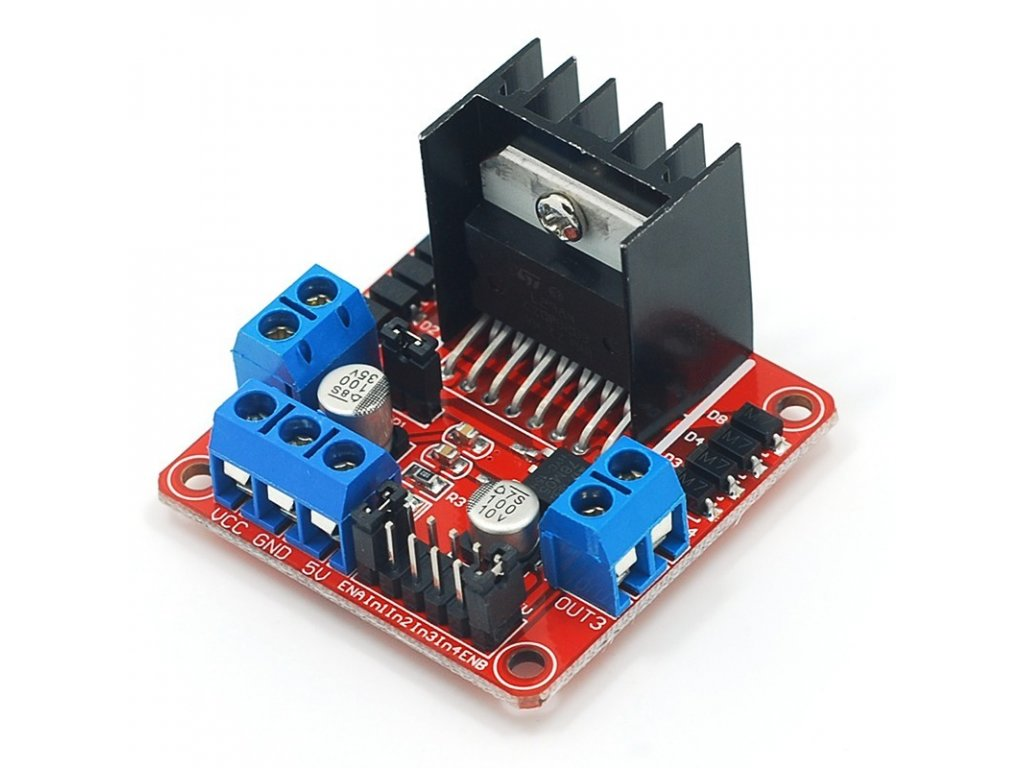
\includegraphics[width=0.7\textwidth]{image/h-mustek.png} %
		\caption{VH-můstek L298N \cite{h-mustek}.} 
	\end{figure}
 
\newpage
\subsection{Servo MG90S 180°}
\noindent Motor Servo MG90S 180° je kompaktní, ale výkonný servomotor široce používaný v různých aplikacích, zejména v oblasti modelování, robotiky a automatizace. Tento motor je schopen otáčet se o 180 stupňů, díky čemuž je neocenitelný ve scénářích vyžadujících přesnou manipulaci s úhly. Já pro svůj projekt ale potřeboval motor s možností otáčení o 360 stupňů, a proto jsem s pomocí pana učitele Godovského provedl úpravy na tomto motoru, aby byl schopen poskytnout požadované otáčení.

	\begin{figure}[ht]
		\centering 
		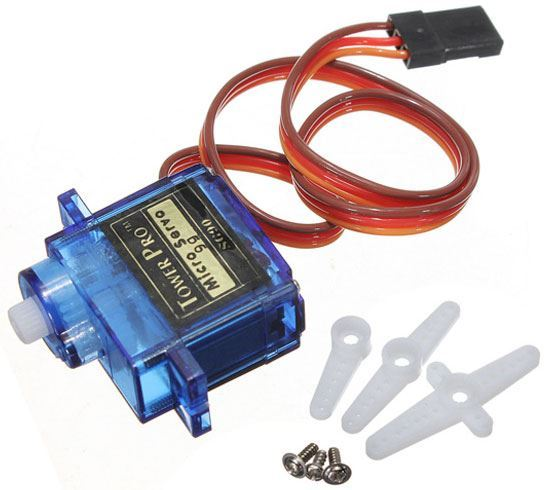
\includegraphics[width=0.4\textwidth]{image/servo.jpg} %
		\caption{Plastové micro servo SG90 9g, 180° \cite{servo}.} 
	\end{figure}

\subsection{Napájení}
\noindent Pro napájení jsem se rozhodl využít čtyři tužkové baterie umístěné v držáku, což mi poskytuje celkové napětí 7 V. Zdroj napájí nepájivé pole odkud pomocí kabelů přivádím proud do vývojové desky a také do H-můstku.

	\vspace*{0.01\textheight}

	\begin{figure}[ht]
		\centering 
		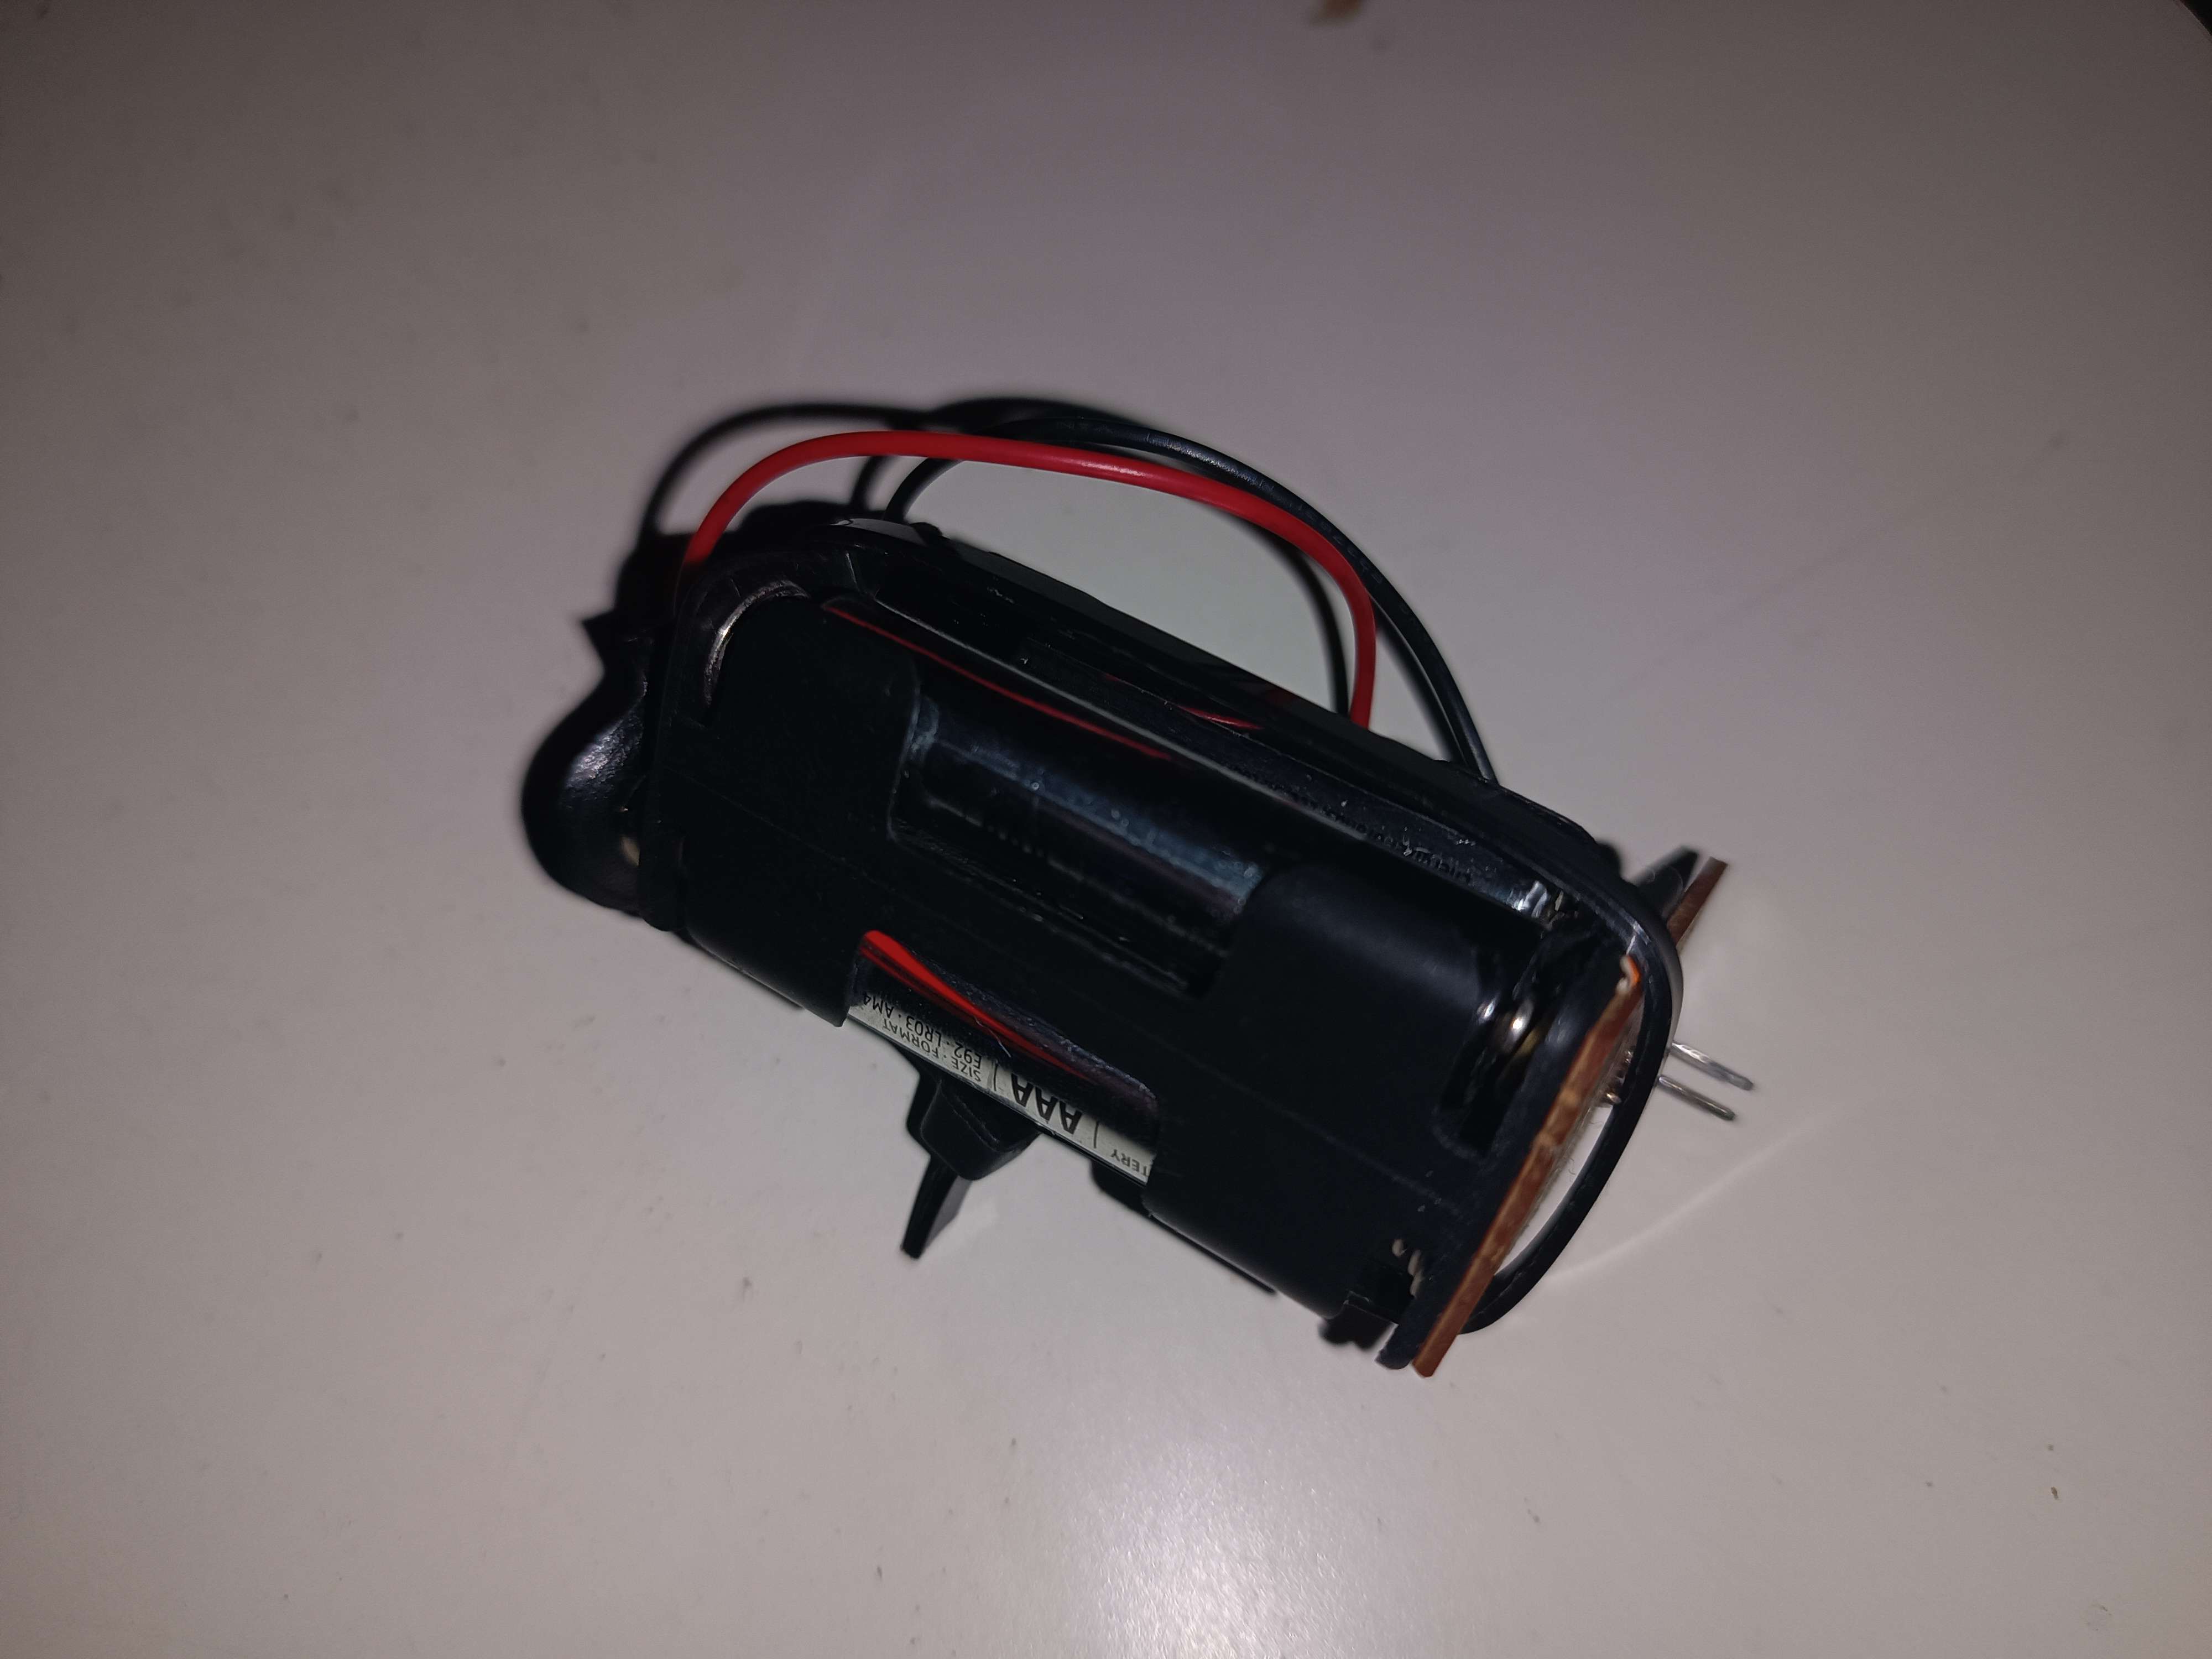
\includegraphics[width=0.4\textwidth]{image/zdroj.jpg} %
		\caption{Napájení pro projekt.} 
	\end{figure}

\newpage
\subsection{Nepájivé pole}
\noindent Nepájivé pole, často nazývané také experimentální nebo prototypovací deska, představuje klíčový nástroj v elektronickém vývoji, a já jsem ho aktivně využíval ve fázi testování mého projektu. Tato deska poskytuje strukturované pole propojovacích otvorů, které umožňují snadné a dočasné připojení elektronických součástek bez nutnosti pájení. To se ukázalo jako neocenitelné zejména v raných fázích projektu, kdy byly potřeba časté úpravy a testování funkčnosti komponentů. Díky nepájivému poli jsem mohl flexibilně experimentovat s různými propojeními, připojovat a odpojovat komponenty a rychle reagovat na změny v návrhu. To nejen zrychlilo proces vývoje, ale také mi umožnilo systematicky ověřit funkčnost jednotlivých součástek.


	\begin{figure}[ht]
		\centering 
		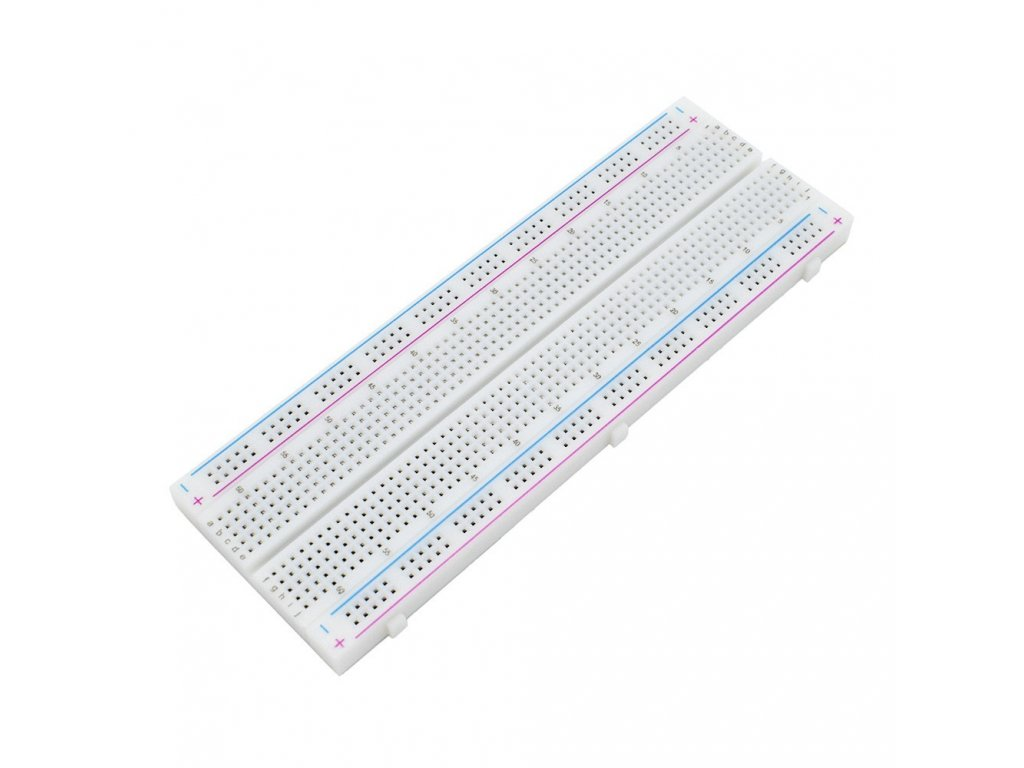
\includegraphics[width=0.6\textwidth]{image/pole.jpg} %
		\caption{Nepájivé pole \cite{pole}.} 
	\end{figure}



\newpage
\section{Software}
\label{sec:prace_s_textem}

V této části bych se rád věnoval programovacímu jazyku Arduino, ve kterém jsem napsal kód pro svůj projekt. Zároveň představím vývojové prostředí PlatformIO, které jsem využil pro snadný vývoj, správu knihoven a ladění aplikace a také věnuji pár slov programu 3DS Max, ve kterém jsem modeloval některé součástky.

\subsection{Programovací jazyk Arduino}
\noindent Arduino je open-source programovací jazyk přímo vytvořen k programování integrovaných obvodů. Postavený na jazyce C++ s rozšířeními pro mikrokontrolery, umožňuje rychlé prototypování a snadnou implementaci elektronických zařízení. Kódy, nazývané "sketche", obsahují funkce setup(), sloužící k inicializaci a loop(), umožňující opakované provádění kódu. Arduino vyniká svou jednoduchou syntaxí a bohatou knihovnou funkcí. Díky aktivní komunitě je snadné sdílet kódy a projekty, což přispívá k jeho popularitě.


\subsection{Vývojové prostředí PlatformIO}
\noindent PlatformIO je integrované vývojové prostředí (IDE) pro vývoj mikrokontrolerových aplikací, včetně těch založených na platformě Arduino. Jeho hlavní výhody zahrnují jednoduchou správu knihoven, snadný přístup k různým platformám a jednotné rozhraní pro vývoj s různými mikrokontrolery. Toto prostředí usnadňuje vytváření, ladění a správu projektů, což z něj činí efektivní nástroj pro rozsáhlý vývoj embedded systémů.




\chapter{Způsoby řešení a použité postupy}
	
\section{Sestavení modelu} 
\noindent Proces sestavování mého tankového modelu byl poměrně namáhavý. Začal jsem tím, že jsem obdržel vymodelované součástky. Jako první jsem se pustil do skládání předních kol, kde jsem pečlivě propojil jednotlivé části a zajistil, aby byly pevně a správně umístěny. Dále jsem spojil dvě hlavní desky podvozku vozidla, čímž mi vznikl základ pro další konstrukci.
Dalším klíčovým krokem bylo zapojení dvou servo motorů do zadní části korby. Tyto motory umožňují  pohyb a ovládání tanku, a tak jsem k nim následně připojil hnací kola, čímž jsem vytvořil pohonný mechanismus vozidla.

\noindent Jako další jsem se věnoval vytváření pásů tanku. Každý z nich se skládal z padesáti jednotlivých dílků, které jsem sestavil a spojil pomocí drobného drátku, který jsem pečlivě provlékl mezi jednotlivými články. Tento proces byl sice detailní, a zabral poměrně dost času ale vytvořil jsem díky tomu opravdu realistický model pásu, bez kterého by se tank neobešel.

\noindent Nakonec zbývalo už jsen nasadit pásy na svá místa, to se ale neobešlo bez problémů. Hnací kola jsou k servo motoru přilepena lepidlem a tudíž jsou docela křehká. Pásy byly udělané tak aby byly mezi koly napnuté a nestalo se, aby nějaký pás vypadl z drážek, to ale zapříčinilo, že se hnací kola pod nátlakem několikrát zkřivila, nebo rovnou odpadla. Rozhodl jsem se tedy pásy o článek rozšířit, což může způsobit, že pásy při jízdě mohou vypadnout.

	\begin{figure}[h]
		\centering 
		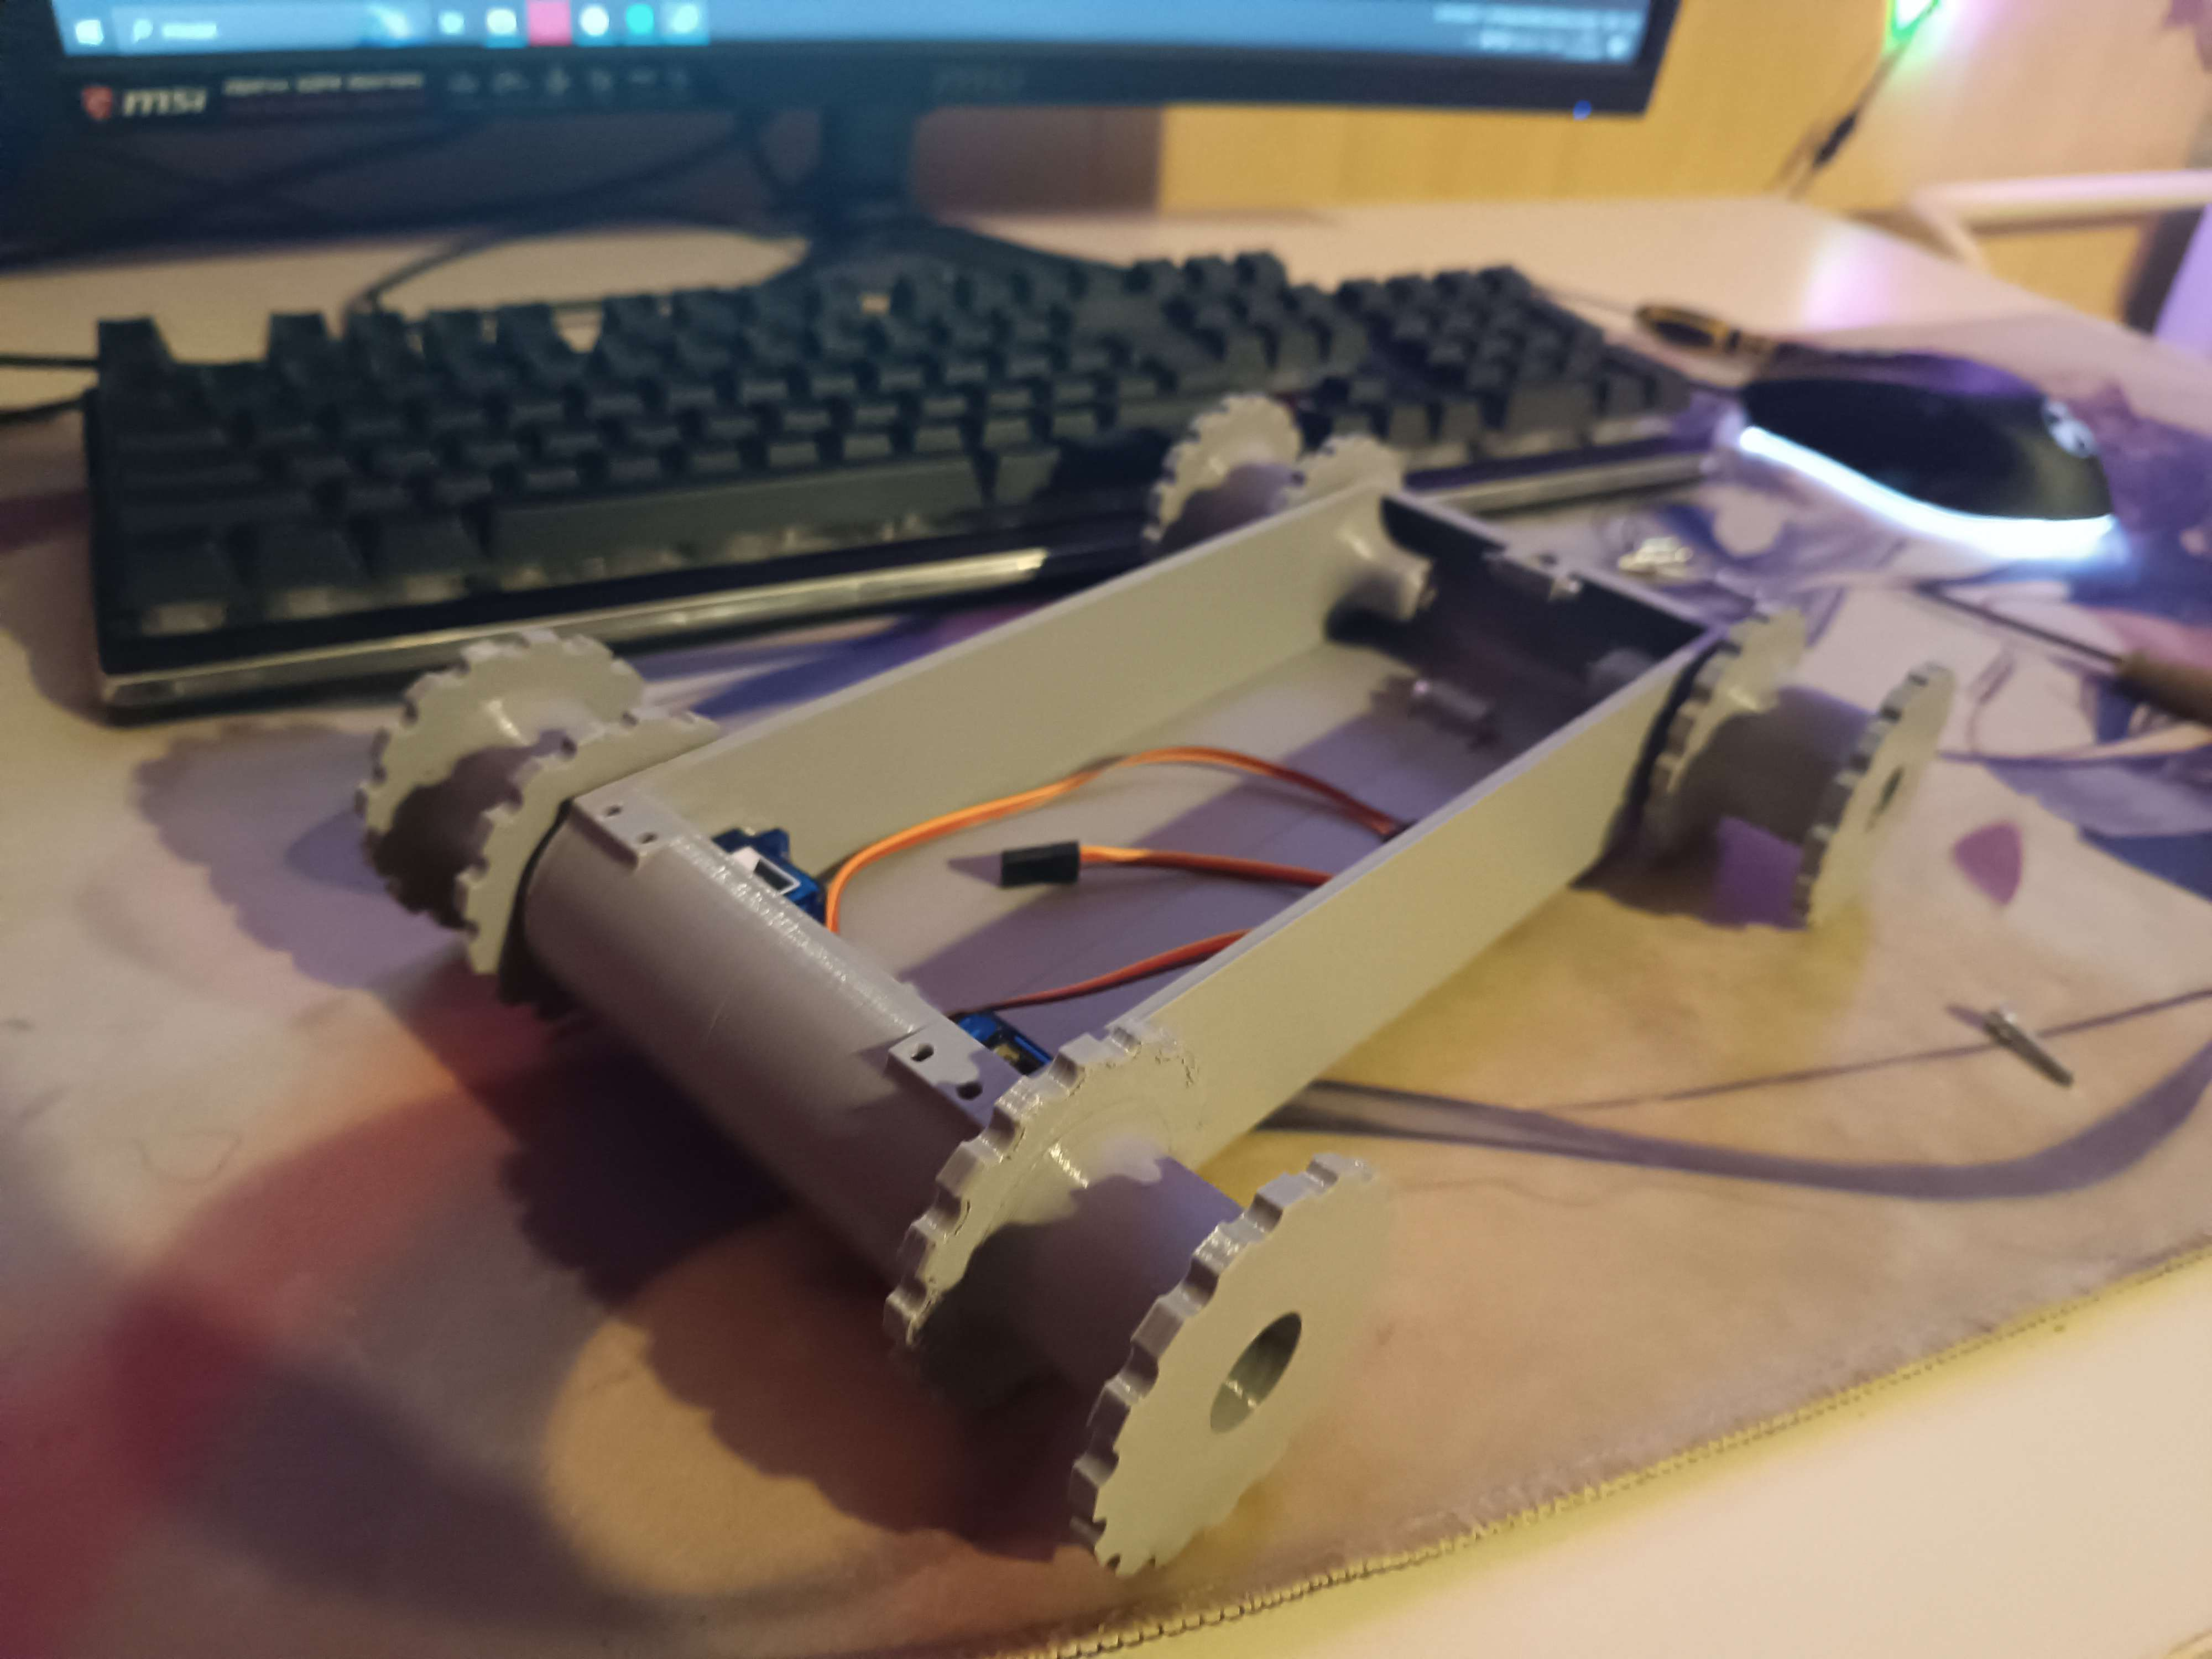
\includegraphics[width=1\textwidth]{image/sestava.jpg} %
		\caption{Sestavený podvozek tanku} 
	\end{figure}

\newpage
 \section{Zapojení a testování součástek}
 \noindent Po sestavení modelu jsem se zaměřil na zapojování součástek do nepájivého pole. Prvním krokem bylo důkladné otestování každé součástky, abych zjistil, zda pracuje tak, jak má. Tento průběžný testovací proces mi umožnil identifikovat případné problémy a zajistit, že každá část mého projektu funguje spolehlivě a bezchybně. Pro nahrávání kódu do vývojové desky ESP32 jsem použil MB programmer, což je štít s USB portem. Tento štít se zapojí přímo do pinů vývojové desky, což usnadňuje konfiguraci a programování. Následně jsem propojil servo motory s H-můstkem, abych ověřil jejich funkčnost. Během této fáze jsem však narazil na problém, když se H-můstek ukázal jako nedostatečně výkonný pro kontrolu obou motorů. V důsledku toho jsem musel nahradit H-můstek silnějším modelem, což vyřešilo problém a umožnilo plné využití servo motorů v mém projektu. 

\newpage
\section{Zprovoznění serveru}
\noindent Pro zprovoznění webového serveru jsem se rozhodl použít knihovny AsyncTCP a ESPAsyncWebServer. Nejdříve jsem integroval knihovnu AsyncTCP, což je asynchronní TCP/IP knihovna, umožňující rychlou a efektivní komunikaci. Tato knihovna poskytuje neblokující komunikaci, což je zásadní pro zachování rychlosti a plynulosti webového serveru.
Dále jsem implementoval knihovnu ESPAsyncWebServer, což je moderní a flexibilní HTTP serverová knihovna pro ESP32. Tato knihovna umožňuje snadné vytváření webových stránek, obsluhu HTTP požadavků a vytváření uživatelsky příjemného rozhraní. Při vývoji serverových funkcí jsem mohl využít asynchronní přístup, což výrazně zvyšuje výkon serveru.

\noindent Nakonec jsem konfiguroval webový server tak, aby poskytoval potřebné funkce pro mé zařízení. To zahrnovalo zpracování HTTP požadavků, ovládání výstupních zařízení, a vytváření dynamických webových stránek. Díky kombinaci těchto knihoven jsem mohl vytvořit responzivní a efektivní webové rozhraní, které je klíčové pro interaktivitu a vzdálené ovládání mého projektu. Celkově tyto knihovny poskytují robustní infrastrukturu pro vytváření webových serverů na platformě ESP32 s důrazem na rychlost, efektivitu a asynchronní komunikaci.

\newpage
 \begin{lstlisting}[style=arduinoStyle]
AsyncWebServer server(80);

void handleRoot(AsyncWebServerRequest *request)
{
  request->send_P(200, "text/html", htmlHomePage);
}

void handleNotFound(AsyncWebServerRequest *request)
{
  request->send(404, "text/plain", "File Not Found");
}

void setup(void)
{
  Serial.begin(115200);

  server.on("/", HTTP_GET, handleRoot);
  server.onNotFound(handleNotFound);

  server.begin();
  Serial.println("HTTP server started");

}
\end{lstlisting}

 \newpage
 
\subsection{Připojení k WiFi}
\noindent Pro dosažení bezdrátové konektivity a propojení s Wi-Fi jsem v projektu využil knihovnu WiFi.h. Tato knihovna poskytuje nezbytné nástroje pro konfiguraci a správu bezdrátového připojení na platformě ESP32. Po integrování knihovny jsem mohl v kódu definovat přístupová jména a hesla k Wi-Fi sítím, ke kterým jsem chtěl, aby se zařízení připojilo. Dále jsem implementoval kód pro inicializaci a připojení k Wi-Fi síti. Tímto způsobem jsem umožnil zařízení komunikovat s okolním prostředím a využívat výhod bezdrátového připojení. 

	\vspace*{0.1\textheight}

 \begin{lstlisting}[style=arduinoStyle]
const char *ssid = "MyWiFiCar";
const char *password = "12345678";

void setup(void)
{
  Serial.begin(115200);

  WiFi.softAP(ssid, password);
  IPAddress IP = WiFi.softAPIP();
  Serial.print("AP IP address: ");
  Serial.println(IP);

  server.on("/", HTTP_GET, handleRoot);
  server.onNotFound(handleNotFound);

  server.begin();
  Serial.println("HTTP server started");

}
\end{lstlisting}

 \newpage
\section{Kód pro ovládání tanku}
\noindent Při navrhování kódu pro ovládání mého tanku jsem systematicky postupoval, abych zajistil přehlednost a efektivitu programu. Začal jsem tím, že jsem přiřadil piny pro každý motor vozidla. Pro každý motor jsem stanovil dva piny, jeden pro jízdu dopředu a druhý pro jízdu dozadu. Abych zvýšil čitelnost kódu a usnadnil případné úpravy, využil jsem globální konstanty pro definici směrů pohybu a stavů motorů. Tyto konstanty poskytují srozumitelný a jednotný zápis v celém kódu. Dále jsem vytvořil funkci rotateMotor, která přijímá číslo motoru a směr otáčení. Tato funkce nastavuje příslušné piny motoru tak, abych dosáhl požadovaného směru pohybu. Pokud je směr FORWARD, motor se nastaví pro jízdu dopředu, pokud je směr BACKWARD, motor se nastaví pro jízdu dozadu, a v ostatních případech jsou oba piny vypnuty, což zastavuje motor.

\vspace*{0.05\textheight}

\begin{lstlisting}[style=arduinoStyle]
void rotateMotor(int motorNumber, int motorDirection)
{
  if (motorDirection == FORWARD)
  {
    digitalWrite(motorPins[motorNumber].pinIN1, HIGH);
    digitalWrite(motorPins[motorNumber].pinIN2, LOW);
  }
  else if (motorDirection == BACKWARD)
  {
    digitalWrite(motorPins[motorNumber].pinIN1, LOW);
    digitalWrite(motorPins[motorNumber].pinIN2, HIGH);
  }
  else
  {
    digitalWrite(motorPins[motorNumber].pinIN1, LOW);
    digitalWrite(motorPins[motorNumber].pinIN2, LOW);
  }
}
}
\end{lstlisting}

\noindent Jako další bylo třeba vytvořit funkci, pomocí které bych definoval samotný pohyb tanku. Vytvořil jsem tedy funkci moveTank, jenž přebírá vstupní hodnotu, která odpovídá pohybu tanku. S využitím předem definovaných konstant pro směry pohybu, jako jsou UP, DOWN, LEFT a RIGHT, tato funkce zajišťuje různé typy pohybů vozidla. V případě, že vstupní hodnota indikuje pohyb nahoru (UP), funkce aktivuje otáčení obou motorů směrem dopředu. Podobně pro pohyb dolů (DOWN) se tank otáčí dozadu. Pro pohyb vpravo (RIGHT) a vlevo (LEFT) dochází ke kombinaci otáčení motorů v odpovídajícím směru. Během návrhu této části kódu jsem dbal na jednoduchost a srozumitelnost, abych usnadnil budoucí úpravy nebo přidání nových funkcionalit.

\vspace*{0.05\textheight}

\begin{lstlisting}[style=arduinoStyle]
void moveTank(int inputValue)
{
  switch (inputValue)
  {
  case UP:
    rotateMotor(RIGHT_MOTOR, FORWARD);
    rotateMotor(LEFT_MOTOR, FORWARD);
    break;
  case DOWN:
    rotateMotor(RIGHT_MOTOR, BACKWARD);
    rotateMotor(LEFT_MOTOR, BACKWARD);
    break;
  case LEFT:
    rotateMotor(RIGHT_MOTOR, FORWARD);
    rotateMotor(LEFT_MOTOR, BACKWARD);
    break;
  case RIGHT:
    rotateMotor(RIGHT_MOTOR, BACKWARD);
    rotateMotor(LEFT_MOTOR, FORWARD);
    break;
  default:
    rotateMotor(RIGHT_MOTOR, STOP);
    rotateMotor(LEFT_MOTOR, STOP);
    break;
  }
}
\end{lstlisting}

 
 
 \section{Webová aplikace}
\noindent Během vytváření webové aplikace bylo mým cílem vytvořit jednoduché webové rozhraní, které by umožnilo nejen ovládání pohybu tanku pomocí tlačítek na webové stránce, ale také sledování živého videa z kamerového modulu. Přestože jsem původně plánoval ukládat HTML kód do samostatného souboru, narazil jsem na omezení mé desky, která neumožňovala pracovat s více soubory. Nakonec jsem se rozhodl uložit veškerý kód pro webový server společně s kódem pro ovládání vozidla do jednoho souboru. Toto omezení mě však motivovalo k pečlivé organizaci a strukturování kódu, aby byl stále přehledný a snadno udržovatelný. 

\noindent Samotný webový server obsahuje minimalistické uživatelské rozhraní upravené s pomocí CSS stylů, video stream z kamery, čtyři tlačítka pro ovládání pohybu tanku a také posuvný slider, který umožňuje plynule nastavit intenzitu světla LED, jež je navržena k osvětlení prostředí v podmínkách nižší osvětlenosti.. Při stisku tlačítka je do funkce pro pohyb vozidla odeslána odpovídající konstanta, která určuje směr pohybu. To umožňuje intuitivní a plynulé ovládání tanku prostřednictvím webového rozhraní.
 

	\chapter{Výsledky řešení}

    \section{Podoba hardwarového zařízení}
\noindent Úplně nakonec jsem se zaměřil na vytvoření designu, který by skryl veškerou elektroniku uvnitř modelu tanku. Pro uzavření jsem vytvořil model horní části korby, poskytující funkční obal pro komponenty. Zdroj energie je umístěn v zadní části korby a prostřednictvím kabelů poskytuje napájení nepájivému poli. Zde je nainstalován H-můstek pro řízení motorů, a přes další soubor kabelů je propojena i deska ESP32 s kamerou. Ta je pevně připevněna ke přední části korby, umožňující snímání obrazu z kamery během pohybu tanku.

\noindent I když jsem spokojen s celkovým vzhledem a umístěním elektroniky, jsou věci které bych v budoucnu chtěl určitě změnit. Z časových důvodů jsem se bohužel nedostal k vymodelování a vytisknutí věže tanku, což bych chtěl ještě ovšem dořešit. Chtěl bych také efektivněji a přehledněji řešit zapojení všech elektrotechnických prvků, jelikož aktuální propojení všech komponentů je poměrně nepřehledné a neestetické. 

    
    \section{Podoba webové aplikace}
    
    Webová aplikace spolehlivě splňuje svůj účel, uživatelé se připojí a monhou tank bez problému ovládat pomocí 4 směrových tlačítek a sledovat při tom živý obraz z kamery tanku. Aplikace je také plně responzivní, lze ji proto používat i na mobilních telefonech nebo tabletech. Do budoucna bych si chtěl s celkový mvzhledem aplikace ještě pohrát a doladit některé nedostatky.
	
	\chapter*{Závěr}
	
    Celkově lze říci, že hlavním záměrem mého projektu bylo vytvořit plně funkční tank s možností dálkového ovládání prostřednictvím webové aplikace nebo ovladače. Většinu cílů, které jsem si stanovil se mi podařilo úspěšně splnit, z čehož mám osobně radost. Z časových důvodů se mi ale bohužel nepodařilo sestrojit ovladač, jako alternativní možnost ovládání. Tuto myšlenku avšak nemám v plánu zahodit a do budoucna bych na ní chtěl určitě ještě zapracovat. Mezi mé další plány na vylepšení projektu patří zprovoznění otáčivé věže, nebo další drobné úpravy vzhledu. Celkově lze tedy říci, že tento projekt byl pro mě nejen technickou výzvou, ale i příležitostí k neustálému zdokonalování a rozšiřování mých znalostí.
	
	%% literatura
	\begin{thebibliography}{99}
		\bibitem{ESP32} \textit{Vývojová deska ESP32} [online]. [cit. 2023-12-29]. Dostupné z: \url{https://bit.ly/vyvojova-deska-esp32-dratek}
		\bibitem{h-mustek}\textit{H-můstek L298N} [online]. [cit. 2023-12-29]. Dostupné z: \url{https://www.laskakit.cz/h-mustek-pro-krokovy-motor-l298n--dualni-motorovy-modul/}
        \bibitem{servo}\textit{Plastové micro servo SG90 9g, 180°} [online]. [cit. 2023-12-29]. Dostupné z: \url{https://www.hadex.cz/l759-servo-plastove-sg90-180-9g-prevody-z-nylonu/}
        \bibitem{pole}\textit{Nepájivé pole} [online]. [cit. 2023-12-29]. Dostupné z: \url{https://www.laskakit.cz/nepajive-kontaktni-pole-830-pinu--bile/}
	\end{thebibliography}
	
	%% obrázky 
	\listoffigures
	
	
	\titleformat{\chapter}[block]{\scshape\bfseries\LARGE}{Příloha \thechapter}{10pt}{\vspace{0pt}}[\vspace{-22pt}] %% nastavení nadpisu u příloh

\end{document}